\documentclass[12pt, twoside, a4paper, openright]{report}\usepackage[]{graphicx}\usepackage[]{color}
%% maxwidth is the original width if it is less than linewidth
%% otherwise use linewidth (to make sure the graphics do not exceed the margin)
\makeatletter
\def\maxwidth{ %
  \ifdim\Gin@nat@width>\linewidth
    \linewidth
  \else
    \Gin@nat@width
  \fi
}
\makeatother

\definecolor{fgcolor}{rgb}{0.345, 0.345, 0.345}
\newcommand{\hlnum}[1]{\textcolor[rgb]{0.686,0.059,0.569}{#1}}%
\newcommand{\hlstr}[1]{\textcolor[rgb]{0.192,0.494,0.8}{#1}}%
\newcommand{\hlcom}[1]{\textcolor[rgb]{0.678,0.584,0.686}{\textit{#1}}}%
\newcommand{\hlopt}[1]{\textcolor[rgb]{0,0,0}{#1}}%
\newcommand{\hlstd}[1]{\textcolor[rgb]{0.345,0.345,0.345}{#1}}%
\newcommand{\hlkwa}[1]{\textcolor[rgb]{0.161,0.373,0.58}{\textbf{#1}}}%
\newcommand{\hlkwb}[1]{\textcolor[rgb]{0.69,0.353,0.396}{#1}}%
\newcommand{\hlkwc}[1]{\textcolor[rgb]{0.333,0.667,0.333}{#1}}%
\newcommand{\hlkwd}[1]{\textcolor[rgb]{0.737,0.353,0.396}{\textbf{#1}}}%

\usepackage{framed}
\makeatletter
\newenvironment{kframe}{%
 \def\at@end@of@kframe{}%
 \ifinner\ifhmode%
  \def\at@end@of@kframe{\end{minipage}}%
  \begin{minipage}{\columnwidth}%
 \fi\fi%
 \def\FrameCommand##1{\hskip\@totalleftmargin \hskip-\fboxsep
 \colorbox{shadecolor}{##1}\hskip-\fboxsep
     % There is no \\@totalrightmargin, so:
     \hskip-\linewidth \hskip-\@totalleftmargin \hskip\columnwidth}%
 \MakeFramed {\advance\hsize-\width
   \@totalleftmargin\z@ \linewidth\hsize
   \@setminipage}}%
 {\par\unskip\endMakeFramed%
 \at@end@of@kframe}
\makeatother

\definecolor{shadecolor}{rgb}{.97, .97, .97}
\definecolor{messagecolor}{rgb}{0, 0, 0}
\definecolor{warningcolor}{rgb}{1, 0, 1}
\definecolor{errorcolor}{rgb}{1, 0, 0}
\newenvironment{knitrout}{}{} % an empty environment to be redefined in TeX

\usepackage{alltt}

\usepackage[utf8]{inputenc}
\usepackage{verbatim}
\usepackage{setspace}
\usepackage{natbib}
\usepackage{enumitem}
\usepackage{tabu}
\usepackage{nth}
\usepackage{graphicx}
\usepackage{epstopdf}
\usepackage{caption}
\usepackage{subcaption}
\usepackage{hyperref}
\usepackage{listings}
\usepackage{float}
\raggedbottom                           % try to avoid widows and orphans
%\sloppy
%\clubpenalty1000%
%\widowpenalty1000%

%\addtolength{\oddsidemargin}{6mm}       % adjust margins
%\addtolength{\evensidemargin}{-8mm}

\renewcommand{\baselinestretch}{1.1}    % adjust line spacing to make
                                        % more readable
\IfFileExists{upquote.sty}{\usepackage{upquote}}{}




\begin{document}
\lstset{language=[Sharp]C}
%%%%%%%%%%%%%%%%%%%%%%%%%%%%%%%%%%%%%%%%%%%%%%%%%%%%%%%%%%%%%%%%%%%%%%%%
% Title

\pagestyle{empty}

\begin{titlepage}

\hfill{\LARGE \bf Neil Satra}

%Vertical center align
\topskip0pt
\vspace*{\fill}

%Horizontal center align
\begin{center}
\begin{doublespacing}


\Huge {\bf Sketching Charts} \\
Computer Science Tripos, Part II \\
Pembroke College \\
\today

\end{doublespacing}
\end{center}

\vspace*{\fill}
\end{titlepage}

\cleardoublepage

\pagestyle{plain}

\setcounter{page}{1}
\chapter*{Proforma}

\begin{tabular}{ll}
Name:               & Neil Satra					\\
College:            & Pembroke College				\\
Project Title:      & Sketching Charts				\\
Examination:        & Computer Science Tripos, Part II, 2014        \\
Word Count:         & TODO							\\
Project Originator: & Alan Blackwell (afb21), Neil Satra (ns532)        \\
Supervisor:         & Alistair Stead (ags46)				\\ 
\end{tabular}

\section*{Original Aims}
This project aims to explore if users are able to create information visualisations faster, or experiment with it more, if given the tools to directly manipulate their charts. Specifically, it involved:
\begin{enumerate}

	\item Building an application that lets users create graphical visualisations of their data by simply sketching their desired output, like they would on paper.

	\item Evaluating the learnability of the interface, and how it compares to existing tools for creating charts, through a user study.

\end{enumerate}

\section*{Work Completed}
I have completed all the core work items by successfully building a Chart component in C\# for Windows applications. This component lets users make a rough sketch of the chart they want to create with a stylus on their tablet, and then uses sketch recognition to create an actual chart based on their data. It performs the sketch recognition by running data mining algorithms on computed features of the digital ink. It also imports data by parsing a user-specified spreadsheet file. I also designed and developed an interface that exposes this component in a user friendly way, attempting to minimize the learning curve by applying Human Computer Interface principles to match the users' mental model through liveness and direct manipulation. I ran a user study assessing how quickly users learnt how to use it (both native and non-native English speakers), and comparing its complexity to that of the existing charting application Microsoft Excel.

As an extension, I implemented the ability to beautify the hand-drawn sketches in a natural-looking manner to match edits made to the chart. I also implemented the ability to erase parts of the hand-drawn sketch, and have those same changes applied to the chart, to further solidify the metaphor to pen and paper.

\section*{Special Difficulties}
%None.
%TODO Shall I put none or the items below?
\begin{itemize}
	\item Acquiring and fixing the source code of a component used for sketch recognition from the team that wrote it.
	\item Automating the testing of the highly visual parts of the project.
\end{itemize}


%\begin{minipage}{\textwidth}
\section*{Declaration of Originality}

I, Neil Satra of Pembroke College, being a candidate for Part II of the Computer Science Tripos, hereby declare that this dissertation and the work described in it are my own work, unaided except as may be specified below, and that the dissertation does not contain material that has already been used to any substantial extent for a comparable purpose.

\bigskip
\leftline{Signed}

\medskip
\leftline{Date}

%\end{minipage}

\clearpage

\tableofcontents

%TODO: Should I include a list of figures here? I really don't see the point

\clearpage


\setcounter{page}{1}
\pagenumbering{arabic}
\pagestyle{headings}

\chapter{Introduction}
\label{cha:introduction}
The aim of this project has been to design and develop Sketchography, an application for users to make a chart of their data by sketching a rough version onto a tablet screen, rather than using a complex Graphical User Interface or programming. The goal is to make an application that's easier for users to pick up than existing charting tools, and one that encourages exploration of the data and various visualisations. I have successfully met all the core requirements, implemented three extensions, and evaluated that the goals were satisfied through a user study.

This chapter documents the motivation for such a project, including previous work in the field, and an overview of what functions the application performs from a user's point of view.

\section{Motivation}
This project is an exploration of Human Computer Interface concepts governing the interactions of users with tools that let them explore and visualise data.

The design of most charting tools is driven by the choice of interface: the mouse and keyboard. Thus, they usually allow graph generation through one of two means:
\begin{enumerate}
\item Configuring a chart template through a number of wizards and dialogue boxes.
\item Manually writing code to generate chart graphics.
\end{enumerate}

Users need to familiarise themselves with how the choices in the wizard, or the commands in the language, translate to graphics.

A better solution is to use a metaphor to a system users have already learnt to use - drawing using pen and paper. Such a system would benefit from matching the users' mental model. 

Additionally, there is a long lag between the users expressing their intention in current systems, and seeing the results of their changes after they close the configuration dialogue or compile and re-run the code. This discourages experimentation and exploration. A better solution would exhibit `liveness' by immediately accommodating users' changes.

\section{Background and Related Work}
Sketching inputs have been studied since the 1960s \citep{sutherland_sketch_1964} as more natural interfaces to computers for graphics-related tasks, compared to indirections like the mouse and keyboard. This has largely been motivated by the widely recognised importance of interactiveness to Information Visualisation (InfoVis) \citep{lee_beyond_2012}. 

Meanwhile, there has been increasing adoption of touch-enabled phones and multi-touch slates amongst the general public, demonstrating people's predilection for what have been referred to as Natural User Interfaces \citep{lee_beyond_2012}. The wide availability of these tools also makes a sketch-based application more feasible to use.


Additionally, \cite{norman_user_1986} describe the `Gulf of Execution', or the gap between a person's intent and their ability to execute that intent. Existing charting tools require users to learn how to accomplish each task, whereas the familiar metaphor of sketching on paper can encourage exploratory work due to the ease of creating changes by visually expressing what sort of change one is trying to make.

There have been a couple of projects that attempt to apply sketch input to the problem domain of creating charts. Microsoft Research's SketchInsight \citep{walny_understanding_2012} lets users make gestures to indicate a type of chart they want. However, by letting the user simply draw the chart they're imagining, rather than making them learn gestures that may not bear a visual resemblance to the end product, Sketchography aims to be easier to learn. Additionally, gestures are immediately converted to charts, which means any further interaction or modifications don't make use of the stylus' digital ink. \cite{chao_poster:_2010} propose a system that lets the user compose basic elements to make visualisations of arbitrary complexity. However, this requires a lot of sketching even for the most basic charts that are commonly used.

In addition to an improved design, this project is also using better sketch recognition techniques, thus reducing the likelihood of frustration due to misclassification of ink strokes.

A larger body of related work is discussed in \autoref{sec:design}, in the context of design decisions made during the implementation of this project.

\section{Project Description}
This paper describes an application that allows the user to sketch a subset of a chart on their computer touch screen as they would on paper. The hypotheses are that, when compared to other charting applications,

\begin{enumerate}
\item[H1] This interface is more `learnable' over time
\item[H2] It encourages exploratory data visualisation creation by making modification easier
\item[H3] Its advantages hold independent of how fluent the user is in English
\end{enumerate}

These hypotheses were investigated through a user study.

The end result is a charting application that works as below:
\begin{enumerate}
\item The user imports data from a Microsoft Excel file.
	\begin{figure}[H]
	\centering
	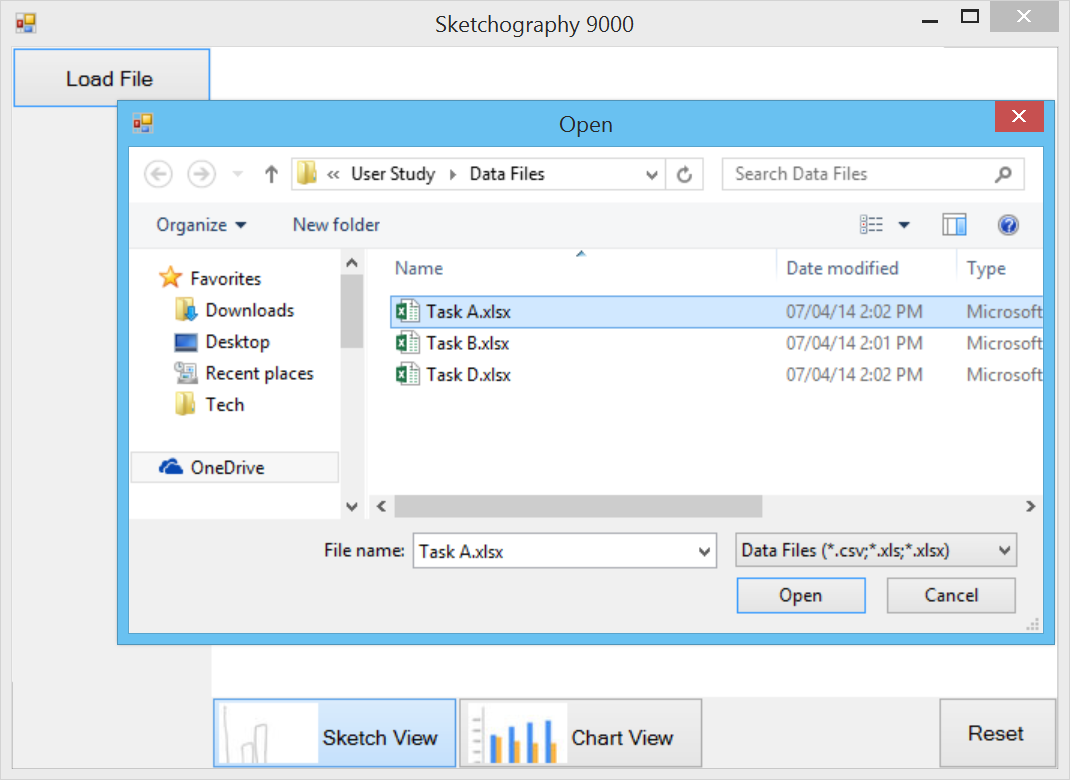
\includegraphics[width=0.6\linewidth]{walk1}
	\end{figure}
\item They sketch a rough indication of a chart.
	\begin{figure}[H]
	\centering
	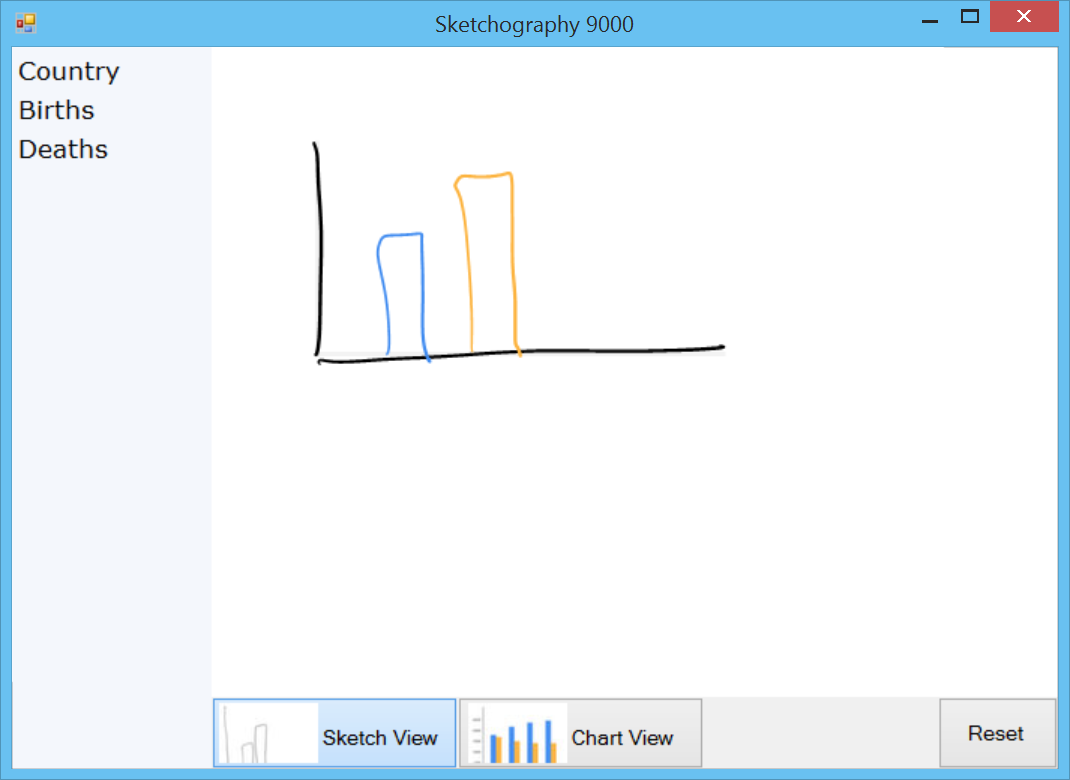
\includegraphics[width=0.6\linewidth]{walk2}
	\end{figure}
\item They drag the data onto elements of the chart to actually bind the data to the chart. 
	\begin{figure}[H]
	\centering
	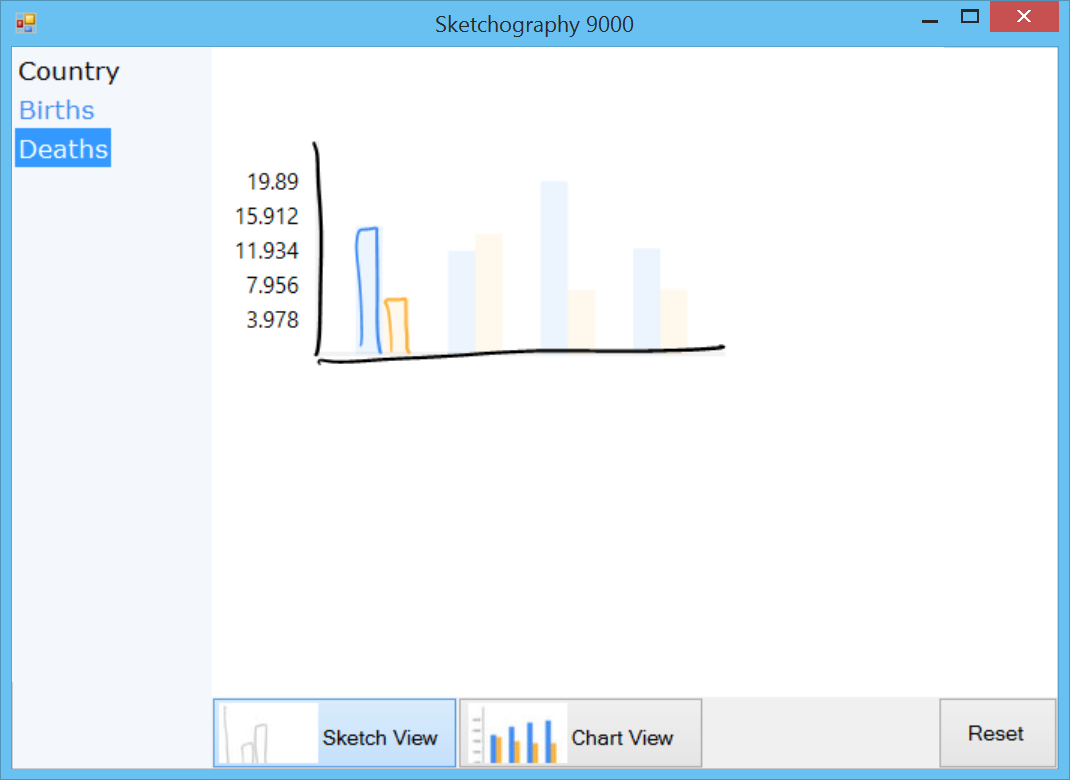
\includegraphics[width=0.6\linewidth]{walk3}
	\end{figure}
\item The tool then creates a 'formal' chart.
	\begin{figure}[H]
	\centering
	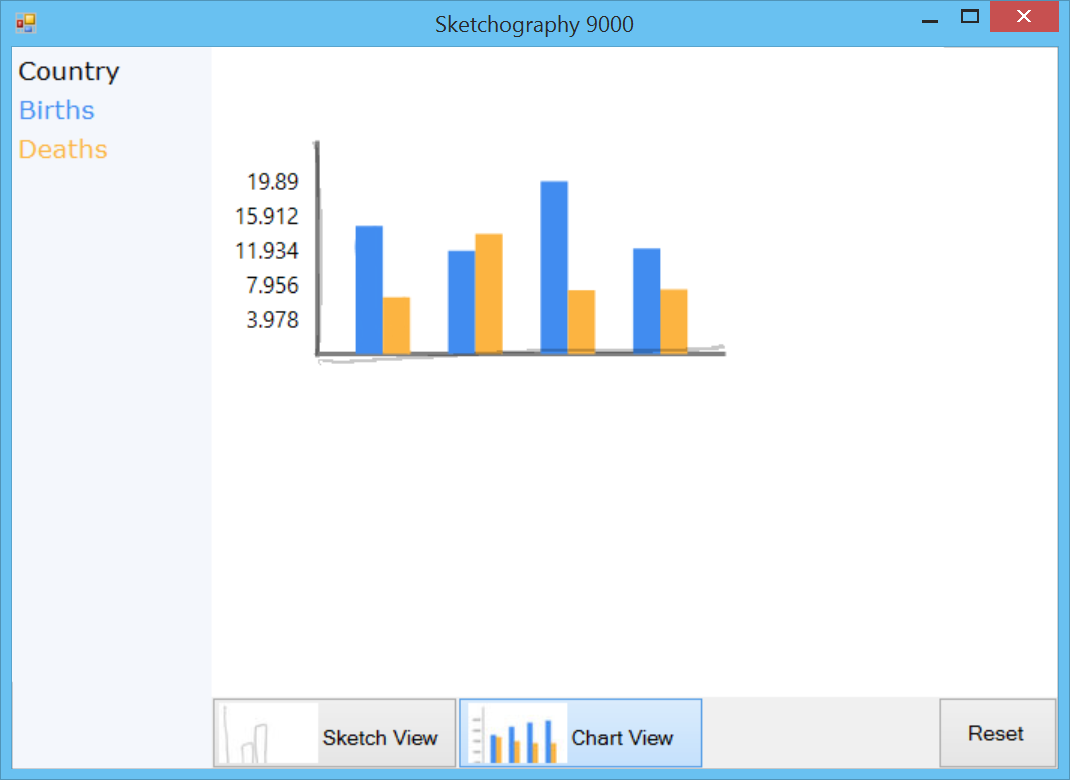
\includegraphics[width=0.6\linewidth]{walk4}
	\end{figure}
\item The tool transforms the user's original sketch to more closely match the formal chart, making the mapping between sketch and formal chart elements evident to the user.
	\begin{figure}[H]
	\centering
	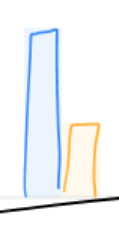
\includegraphics[width=0.1\linewidth]{walk5}
	\end{figure}
\item Any changes on either the sketch or formal chart is fed through to the other view. For example, erasing the a sketched bar removes a data series from the formal bar.
	\begin{figure}[H]
	\centering
	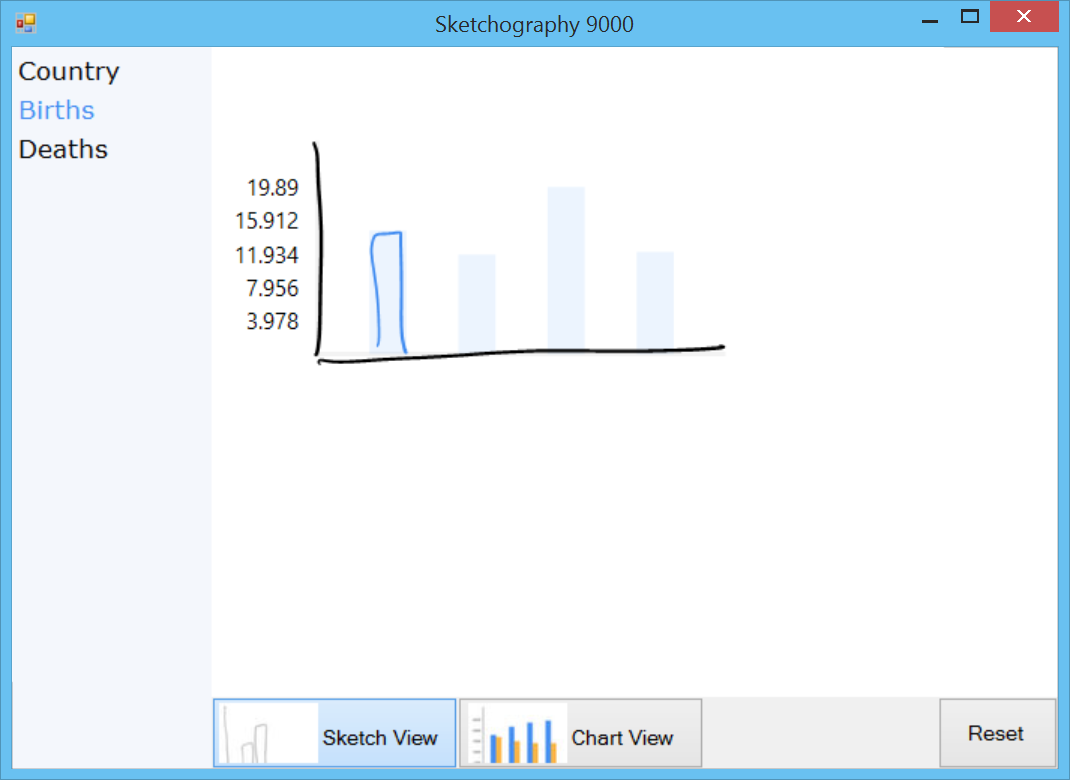
\includegraphics[width=0.6\linewidth]{walk6}
	\end{figure}
\end{enumerate}

\section{Summary}
Existing charting tools are very capable and full-featured, but aren't as easy to learn as they should be, in order to encourage users to explore the data. A new application was proposed that should be easy to learn, and make modifications of the data easy. It uses well-performing data mining algorithms to perform ink stroke recognition, and a charting component to display the data visually. A user study was carried out to confirm that it achieved its goals.

\chapter{Preparation}
This project involved vast exploratory design work, in preparation of the actual implementation.

	\section{Requirements}
	This project could go in numerous different design directions from the start. Since the functionality and its benefits over existing systems depended heavily on the design chosen, it was hard to separate what benefits the program would achieve from what features the program would include and how it would expose them to the user. 
	
	However, in order to focus our exploration and make sure that the focus was on achieving some real deliverables for end users, a requirement analysis was necessary. The following functional goals were listed based on the project proposal, which focus on what basic tasks the system must help the user achieve, while allowing leeway in how the program exposed and implemented these features.
	
	The system must allow the user to:
	\begin{enumerate}[label=\bfseries Core \arabic*:]
		\item Use any data they have in reasonably arranged formats in common file types.
		\item Specify the type of chart they want by drawing a likeness of it on screen using a stylus.
		\item Bind the data to the chart using an interface that makes it clear how the data is affecting the visualisation.
		\item Specify visual, size and positioning properties of the chart through the sketches.
		\item Manipulate the visual appearance of the created chart.
	\end{enumerate}
	
	In addition, time permitting, the system may:
	\begin{enumerate}[label=\bfseries Extension \arabic*:]
		\item Transform user-drawn sketches to show the visual link to the formal chart elements.
		\item Feed back manipulations applied to the formal layer back to the user drawn sketches, in order to keep the visuals of the formal and sketch layers in synchronisation.
		\item Allow users to undo actions by erasing sketches, and remove the corresponding formal elements without throwing errors.
		\item Allow users to manipulate any property of chart elements, not just one, so that the domain of visualisations they can create is infinite. For example, allow them to bind not just the height of bars in a bar chart to data, but also their width and colour. 
		\item Analyse the data and infer properties that may allow it to automatically suggest properties of the chart, such as which field belongs on which axis, or whether a data series should be log scale or linear scale.
		\item The user must be able to export the chart as a Microsoft Chart object that can be embedded as a dynamic object in Microsoft Office files, not just as a raster image.
	\end{enumerate}
	
	The core of this project focusses on making more usable software, rather than providing additional functionality, compared to existing systems. Hence, some usability goals were also specified:
	\begin{enumerate}[label=\bfseries Usability \arabic*:]
		\item Users must be able to create charts at least as quickly as they can using current systems.
		\item Users must be able to build a mental model of the software's behaviour within 2 uses of it. They should thus be able to accurately predict the consequences of any action taken within the software.
		\item Changes to the information visualisation must occur through directly manipulating the visual representation of the chart, rather than through disconnected User Interface widgets.
		\item The user must be able to easily try out changes to the visualisation, see what that would look like, and undo them if needed.
	\end{enumerate}
	
	\section{Design Goals}
	In order to meet the usability requirements, some design principles need to be followed. 
	%TODO Talk about Direct Manipulation in detail.
	
	
	
	\section{Work Items}
	An iterative development process, similar to the Spiral Model was adopted for this project. This allowed early experimentation with and user testing of the various components and different interface designs. The following broad work items were identified as necessary to achieve the objectives above:
	%TODO Maybe insert a picture of my development process here, including the user studies?
	\begin{enumerate}
		\item Get the requisite approvals for the human study from the Ethics Review Committee.
		\item Assess the various methods to build a classifier for ink recognition, including using the RATA Framework.
		\item Run an initial user study to  see how people naturally draw graphs, and also use it to collect training examples for the classifier.
		\item Build a UI that accepts strokes, runs them through the classifier, and shows the user feedback to indicate successful recognition.
		\item Build the UI widget that lets users import their spreadsheets in Microsoft Excel (xlsx) or Comma Separated Value (csv) files. It must then expose the various fields detected.
		\item Build the charting component to convert the recognised sketches and the ink into a finished visualisation.
		\item Run a pilot study followed by a user study to evaluate the system.
	\end{enumerate}
	
	
	\section{Development Environment}
	For this project, the hardware available was a Microsoft Surface Pro (\nth{1} gen), which features the active digitizer screen required for precise inking. Since this machine runs Windows by default, we chose to develop the system using the .NET framework, which has built-in support for Tablet PCs and Ink handling.
	
	As a precaution, insurance was taken out on the machine to ensure quick replacement in case of damage or loss. Additionally, version control was used extensively in the project, to ensure no work was lost. The code for the RATA ink stroke recogniser, described below, was uploaded to a Git repository in collaboration with RATA's authors. The code for this project was then written in a fork of that repository, to allow updates to RATA to be pulled in. The dissertation itself was written in \LaTeX , so that the text files could be versioned in another Git repository. Both repositories were backed up off-site on repository host Bitbucket. The dissertation was also backed up online using file synchronisation software Microsoft OneDrive. 
	
	\section{Building the classifier}	
	Core to the system is an ink recognition component that identifies the chart element (e.g.\ bar, axis) that the user has sketched. This must work above a certain accuracy threshold or the system will prove frustrating to users \citep{frankish_recognition_1995}. However, since the project scope included other components too, the time available to build this classifier was limited. Additionally, given the complexity of building a classifier, and our limited experience with building them, it would be difficult to get the same accuracy as those provided in a mature library. Hence, we decided to build a classifier using existing tools rather than implementing one from scratch. 
	
	\subsection{Recognition Method}
	A number of different approaches have been taken in building systems that automatically interpret hand-drawn sketches. These approaches vary in the recognition accuracy they offer, and the robustness to generalise across multiple domains. \citep{ouyang_visual_2009}. Some of the approaches that have been attempted:
	
	\begin{itemize}
		\item Focus on \textbf{defining shapes structurally}. A base vocabulary of primitives like lines, ellipses and arcs is built by describing the properties of such shapes. \citep{shilman_statistical_2002} used a hand-coded grammar to describe shapes in a domain as a composition of such primitives. \citep{alvarado_sketchread:_2004} used dynamically constructed Bayesian networks to scale this process to multiple domains. \citep{hammond_ladder:_2006} developed a language to manually describe how diagrams in a domain are drawn, displayed and edited. 
		\item Look at the \textbf{visual appearance} of shapes and symbols. \citep{kara_image-based_2004} used image-based similarity metrics to perform template matching. \citep{shilman_recognition_2004} broke up the ink into connected subgraphs of nearby strokes, which were then compared to known symbols. \citep{oltmans_envisioning_2007} proposed a visual parts-based method that utilise a library of shape contexts to describe and identify symbols in a domain.
		\item \textbf{Compute features} of the ink. \citep{patel_ink_2007} selects these features and sets their thresholds statistically. \citep{yu_domain-independent_2003} uses heuristics for the same purpose. \citep{chang_rata._2010,  rubine_specifying_1991, willems_iconic_2009} all use machine learning to automatically find relationships between features and choose an appropriate feature set accordingly.
	\end{itemize}		
	
	\citep{chang_rata._2010} showed that the first two approaches forego some accuracy, since they rely on the final pixel values of the sketch and so do not fully exploit the rich temporal data stored with digital ink. Within the last approach, they showed that using machine learning allows recognisers to be generated for new domains with less effort than statistical or heuristic methods. Since the domain for this charting application could grow over time, we wanted a recogniser that could be adapted easily over time. Using data mining, this can be done using training data rather than programming effort.
	
	Having decided on using a feature-based approach that selects the feature set by data mining a training dataset, there were a number of alternatives available to us. While most projects, like \citep{rubine_specifying_1991} and \citep{willems_iconic_2009}, rely on one or two data mining algorithms, \citep{chang_rata._2010}'s RATA.SSR combines the results from four well-performing algorithms in WEKA \citep{hall_weka_2009} tuned to their best configurations, to provide a more accurate recogniser. RATA.SSR thus outperformed all the other recognisers tested (PaleoSketch \citep{paulson_paleosketch:_2008}, CALI \citep{fonseca_cali:_2002}, \$1 recogniser \citep{wobbrock_gestures_2007}) on domains other than the one they were explicitly demonstrated on. 
	
	Besides, RATA.SSR also has the advantaged of outputting an API that can be plugged into our system after we build the recogniser. Additionally, one of the authors, Beryl Plimmer, previously worked with some members of the Graphics and Interaction Group at the Cambridge Computer Laboratory, and so could be reached for support and source code, which proved to be an invaluable resource.
	
	\subsection{Data collection}
	After acquiring RATA, we inspected the code and did manual testing, which revealed some blocking bugs. Since we were in contact with the authors of the software, we were able to confirm with them that these were indeed bugs. We implemented fixes for them and contributed them back to the authors, and are working towards getting the code ready for to be published Open Source.
	
	With a working version of RATA, an initial study was run to collect training data. We asked 10 participants (20-26 year old Cambridge students, studying a large variety of subjects) to draw a chart. I spoke out the following prompt:
	
	\begin{quotation}
	Imagine you are a government official trying to use a bar chart to visualise how the population has grown over time. Can you sketch out what this bar chart might look like? Just treat this screen like paper.
	\end{quotation}
	
	 They were then presented a simple UI with a large white canvas and the following task description written in a panel:
	
	\begin{quotation}
	Draw 2 axes. Label the x axis 'Year' and the y 'Population'. Draw 3 bars of different heights. Each shape (axis, bar) should be drawn in one stroke.
	\end{quotation}
	
%	First, they were shown a spreadsheet file containing sample data as below:
%	\begin{tabu}{l r r}
%		\rowfont{\bfseries} Year & Births & Deaths \\
%		2010 & 50,000 & 30,000 \\
%		2011 & 40,000 & 35,000 \\
%		2012 & 36,000 & 37,000 \\
%		2013 & 34,000 & 35,000 \\
%	\end{tabu}
%	
%	\vspace{10pt}
%	
%	Next, I spoke out the following task prompt.
%
%	
%	\begin{quote}
%		Say you are a government official trying to visualise trends in birth and death rates over time. Could you draw a bar hart on this screen that you would need to visualise this. No need to plot the actual data, just a rough sketch of what this chart would look like.	
%	\end{quote}
	
	They were asked to draw the same chart 2 times, in order to get 20 training samples in total, and to observe how much variation there is between multiple sketches by the same user. On the second drawing, they were encouraged to draw a less conventional chart, to make the system as robust in the face of variations as possible. 
	%TODO ^Explain this better
		
	\begin{figure}[h]
        \centering
        \begin{subfigure}[b]{0.5\textwidth}
                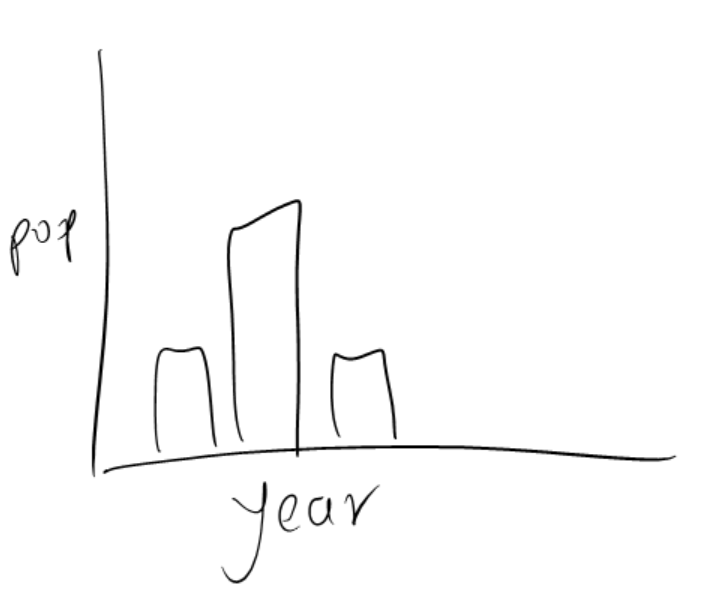
\includegraphics[width=\textwidth]{collection1}
                \caption{Regular chart}
                \label{fig:regular}
        \end{subfigure}%
        ~ %add desired spacing between images, e. g. ~, \quad, \qquad etc.
          %(or a blank line to force the subfigure onto a new line)
        \begin{subfigure}[b]{0.5\textwidth}
                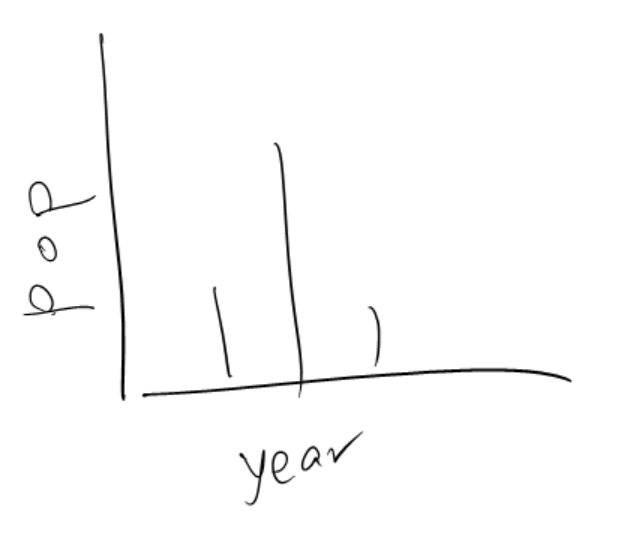
\includegraphics[width=\textwidth]{collection2}
                \caption{Using lines instead of bars}
                \label{fig:lines}
        \end{subfigure}
        ~ %add desired spacing between images, e. g. ~, \quad, \qquad etc.
          %(or a blank line to force the subfigure onto a new line)
          \begin{subfigure}[b]{0.5\textwidth}
                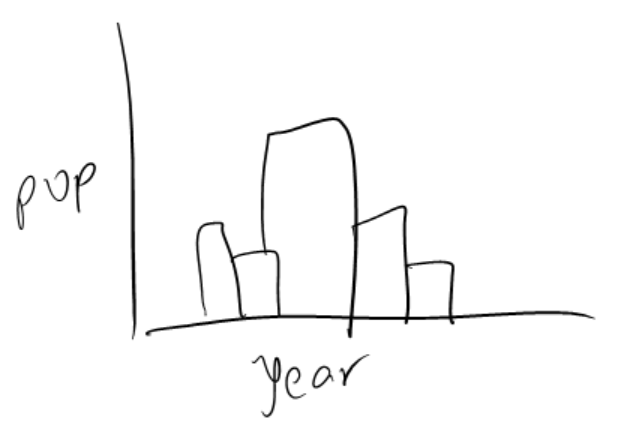
\includegraphics[width=\textwidth]{collection3}
                \caption{Grouped bars}
                \label{fig:grouped}
        \end{subfigure}%
        ~ %add desired spacing between images, e. g. ~, \quad, \qquad etc.
          %(or a blank line to force the subfigure onto a new line)
        \begin{subfigure}[b]{0.5\textwidth}
                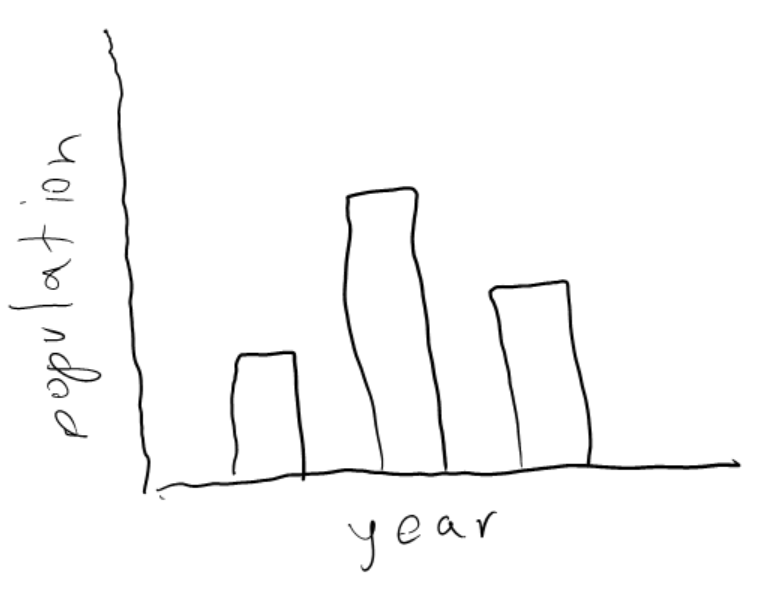
\includegraphics[width=\textwidth]{collection4}
                \caption{Using a mouse instead of the stylus}
                \label{fig:trembling}
        \end{subfigure}
        ~ %add desired spacing between images, e. g. ~, \quad, \qquad etc.
          %(or a blank line to force the subfigure onto a new line)
        \caption{Some of the more unusual chart sketches collected}\label{fig:data_collection_samples}
	\end{figure}
	
	Three elements were then defined: Axis, Bar and Text (an extra element, 'L Axis' was added later based on feedback from a pilot user study). We went through each figure and labelled the various elements.
	
	\begin{figure}[h]
		\centering
		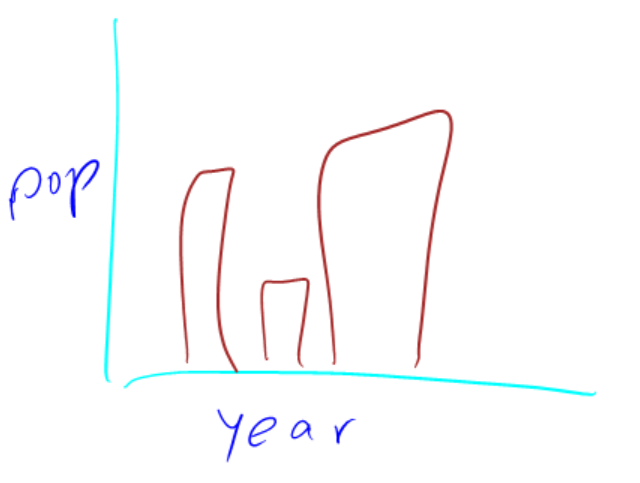
\includegraphics[width=0.5\textwidth]{collection_labelled}
		\caption{Elements of the sketch labelled as Axis (cyan), Bar (brown) or Text (dark blue)}
		\label{fig:collection_labelled}
	\end{figure}

	Once all the elements in all the charts were labelled, we could begin training. RATA includes a dataset generator tool that allowed easy extraction of various features of the strokes, such as 'distance from first to last point', 'absolute curve of largest segment' and 'pressure variation'. Data for 121 such attributes, about 270 ink strokes was compiled into a .csv file for use in training. 
	\subsection{Training}	
	The labelled data was then sent to a 'Vote' classifier in Weka, which combines the probability distributions derived from multiple classifiers \citep{kuncheva_combining_2004}. Specifically, the types of classifiers combined were Logit Boost, Bayes Net, LMT (Logistic Model Trees) and Random Forest. In order to assess how well each of these individual classifiers were performing, an experiment was set up using Weka Experimenter. The data collected in the initial study was shuffled, and then 66\% was chosen randomly as training data, the rest as testing. Then a paired T Test gave the following results:
	
	%TODO Make this all stay together as much as possible.

\vspace{10pt}
Tester:     Paired Corrected T Tester

Analysing:  Percent correct

Confidence: 0.05 (two tailed)

%\begin{table}[thb]
%
%%\scriptsize
%{\centering
%\begin{tabular}{c p{0.9 \textwidth}}\\
%(1) & meta.LogitBoost '-P 100 -F 0 -R 1 -L -1.7976931348623157E308 -H 1.0 -S 1 -I 10 -W trees.DecisionStump' 8627452775249625582 \\
%(2) & bayes.BayesNet '-D -Q bayes.net.search.local.TAN -- -S BAYES -E bayes.net.estimate.SimpleEstimator -- -A 0.5' 746037443258775954 \\
%(3) & trees.LMT '-P -I 50 -M 200 -W 0.0 -A' -1113212459618104943 \\
%(4) & trees.RandomForest '-I 100 -K 0 -S 1' -2260823972777004705 \\
%\end{tabular}
%}
%\caption{\label{}Classifier Algorithms Used}
%\end{table}

%\begin{table}[h]

%\footnotesize
%{\centering \begin{tabular}{lrr@{\hspace{0.1cm}}cr@{\hspace{0.1cm}}cr@{\hspace{0.1cm}}c}
%\\
%\hline
%Dataset & LogitBoost & BayesNet & & LMT & & RandomForest & \\
%\hline
%Initial study & 97.05 & 98.15 &         & 98.80 &         & 96.07 &        \\
%\hline
%\multicolumn{8}{c}{$\circ$, $\bullet$ statistically significant improvement or degradation}\\
%\end{tabular}  \par}
%\caption{\label{}Comparison of accuracy of the algorithms used}
%\end{table}


\begin{table}[h]
\centering
\begin{tabular}{l c}
\textbf{Algorithm} & \textbf{Accuracy} \\
LogitBoost 	&	97.05 \\
BayesNet 	&	98.15 \\
LMT			&	98.80 \\
RandomForest &	96.07 \\

\end{tabular}
\caption{Comparison of accuracy of the algorithms used}
\end{table}





\chapter{Implementation}
\section{Design}
	Now that we had shown that a classifier could be built with relatively small sets of training data that still performed well, we had to design the interface to expose this functionality. This largely involved assessing tradeoffs between choices.
	
	\subsection{`Sketchy' or Formal}	
	\begin{figure}[h]
		\centering
		\begin{subfigure}[b]{0.4\textwidth}
			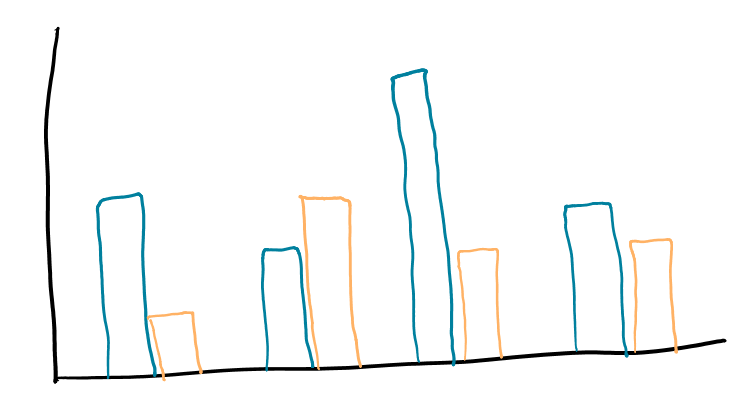
\includegraphics[width=\textwidth]{sketchy}
			\caption{Sketchy look}
			\label{fig:sketchy}
		\end{subfigure}
		\begin{subfigure}[b]{0.4\textwidth}
			\includegraphics[width=\textwidth]{formal}
			\caption{Formal look}
			\label{fig:formal}
		\end{subfigure}
	\end{figure}
	User content can be in shown in two styles: sketch or formal. This refers to the usability dimension described by \cite{bresciani_collaborative_2008} as 'Perceived Finishedness'. \cite{yeung_effect_2008} showed that a doodle-like appearance of low-fidelity prototypes encourages early-stage experimentation and discussion, whereas a formal appearance looks finished and professional.  Thus, we had to choose whether the system should generate the rest of the chart with a 'sketchy' look, or convert the input into a finished chart with a formal look. \cite{blackwell_formality_2008} note how the rapid replacement of pen and paper by computers has made more of our processes formal and precise, potentially discouraging us from exploration and iteration in creative processes that would benefit from them.
	
	Generating the 'sketchy' look can be non-trivial, \citep{plimmer_sketchnode:_2010, wang_sketchset:_2011} e.g.\ if the user draws one bar, how should the system generate more bars that look hand-drawn by the same author but not just like stretched versions of the first bar? Additionally, if the users want to present these charts to an audience, they must look polished, and so at some point an export option for a formal look needs to be offered. Thus, we decided to offer a hybrid that shows the user's input in sketch form, with the system's output in formal form. Extensions were implemented to keep these two forms as closely in synchronization as possible, thus making the mapping visually evident.
	
	\subsection{Sketches or gestures}
	A related design decision was whether to use sketches or gestures. Sketches share some visual semblance with the chart they're trying to indicate, whereas gestures are just movements chosen from a library of easy-to-distinguish movements, that behave like commands instructing the software to choose a certain chart type. SketchInsight \citep{walny_understanding_2012} uses the latter approach, requiring just an `L' shape to indicate a bar chart, or a `V' shape to indicate a line chart. 
	
%		\begin{tabular}[h]{p{0.5 \linewidth} | p {0.5 \linewidth}}
%			\bfseries{Pros} & \bfseries{Cons} \\
%			This would provide higher recognition accuracy, since the domain of shapes to distinguish between is limited, and can be designed to maximise differences between them. & One of the principles of direct manipulation is to avoid using a command language, but a gesture library is exactly that, requiring users to remember which gesture corresponds to which chart type or element. \\ \hline
%			& A gesture is transient, unlike a sketch. Users wouldn't be able to modify their input, they would have to redo their actions. 
%		\end{tabular}	
		
			\textbf{Pros}
			\begin{itemize}
			\item This would provide higher recognition accuracy, since the domain of shapes to distinguish between is limited, and can be designed to maximise differences between them. 
			\end{itemize}
			
			
			\textbf{Cons} 
			\begin{itemize}
			\item A gesture is transient, unlike a sketch. Users wouldn't be able to modify their input, they would have to redo their actions. 
			\item One of the principles of direct manipulation is to avoid using a command language, but a gesture library is exactly that, requiring users to remember which gesture corresponds to which chart type or element. 
			\end{itemize}
				
	
	This would provide higher recognition accuracy, since the domain of shapes to distinguish is much more limited, and can be designed to maximise differences between them. 
	
	% Can cite Chao
	\subsection{Modes or modeless}
	Since the application now has both sketch and formal content, the user must have an easy way to switch between the two views. One approach is to give the user an explicit UI widget to toggle between the two modes. This way, the user explicitly indicates what they want to see, and thus should have a better understanding of what state the system is in. This also allows the system a chance to change the controls available to the user.
	
	The other approach is to avoid modes, requiring lesser cognitive effort from the user since they don't need to keep track of what state the system is in. In this project, this could have been done by showing the sketch view when the user was about to edit the chart. The active digitizer hardware allows the system to detect when the user brings the stylus within range of the screen, just before they actually touch the screen, allowing the chart to be in sketch view by the time the stylus is down. When the stylus goes out of range, the system can switch to the formal chart view. This would solidify the metaphor that edits are done to the sketch, but the final product to be looked at is the formal view. 
	
	At first, the modeless version was chosen for its lower cognitive overhead. However, when the extension to allow edits not just to the sketch view, but also the formal view, was undertaken, we had to switch over to a mode-based system to allow the user to interact with the graph in both views with their stylus.
	
	\subsection{Standard or custom charting widget}	
	Since the system is generating a formal version of the chart, a charting component is required to render this visualisation. The .NET framework comes with built-in chart controls that offer basic functionality with relatively low implementation effort. They also allow easy export as dynamic chart objects into Microsoft Office files. However, customising their appearance beyond a certain point is extremely difficult, making it easier to just make one's own charting component from scratch and control all aspects of the rendering. This means having to re-implement a lot of core functionality though, such as scaling shapes correctly, choosing labels that are round figures when possible, and generating colours than work well together for different data series. This also means that the chart can only be exported as a raster image rather than as a chart object.
	
	To enable rapid prototyping, we chose to utilise the standard charting component at first. As our needs to customise the chart grew, we were able to make our own chart class that implemented the same interface as the standard component, and so could be slotted in to replace it.
	
	\subsection{Finite or infinite domain}
	Some tools, such as Microsoft Excel, let the user make one of a limited set of charts, such as bar or pie charts, quickly. Others, (which usually involve coding), such as D3.js, let the user make a vast variety of visualisations by creatively combining basic elements like lines, boxes and wedges. However, these require expert knowledge of the tools, and take longer to create basic visualisations. 
	
	\begin{table}[h]
	\begin{tabular}{p{0.5 \linewidth} p {0.5 \linewidth}}
	\bfseries Library of charts 	& \bfseries Modular charts \\
	Draw basic gestures or elements to indicate which chart type is desired & Draw any one of 7 basic components (lines, bars, labels etc) and bind data to attributes of theirs such as width, height, colour or radius \\
	Finite domain 		& Infinite domain \\
	Quick				& Slower \\
	Simple interface, just drop data on an element to bind data	& Complex interface to expose all attributes and manage data binding \\
	\end{tabular}
	\end{table}
	
	\citep{chao_poster:_2010} uses pen gestures to indicate 'proto-objects' that can be combined. While an infinite domain system that uses pen sketches would have been intriguing to explore, it would contradict the project's primary usability goal that the system should be faster than users' current systems. Additionally, the 80/20 rule indicated that while a few power users may want to generate custom visualisations, the majority would just want to make simple charts. Thus, the additional functionality didn't justify the additional complexity for the average user.
	
%	\subsection{To beautify or not to beautify}
%	The formal graphics generated by the system are easy to modify with existing tooling, whereas human ink strokes are less straightforward to modify while maintaining their natural look and feel.


	\section{Development}
	Interleaved with the design process above was the development process detailed in this section. The C\# code supports a stand-alone Sketch Chart component that can be used in any Windows Forms application that requires charting functionality, as well as a reference implementation of such an application, Sketchography, which lets users import their Microsoft Excel or Comma Separated Values data and generate charts. This satisfies all the core requirements described in \autoref{sec:Requirements}, as well as 3 of the 6 extensions outlined.
	
	\begin{figure}[h]
		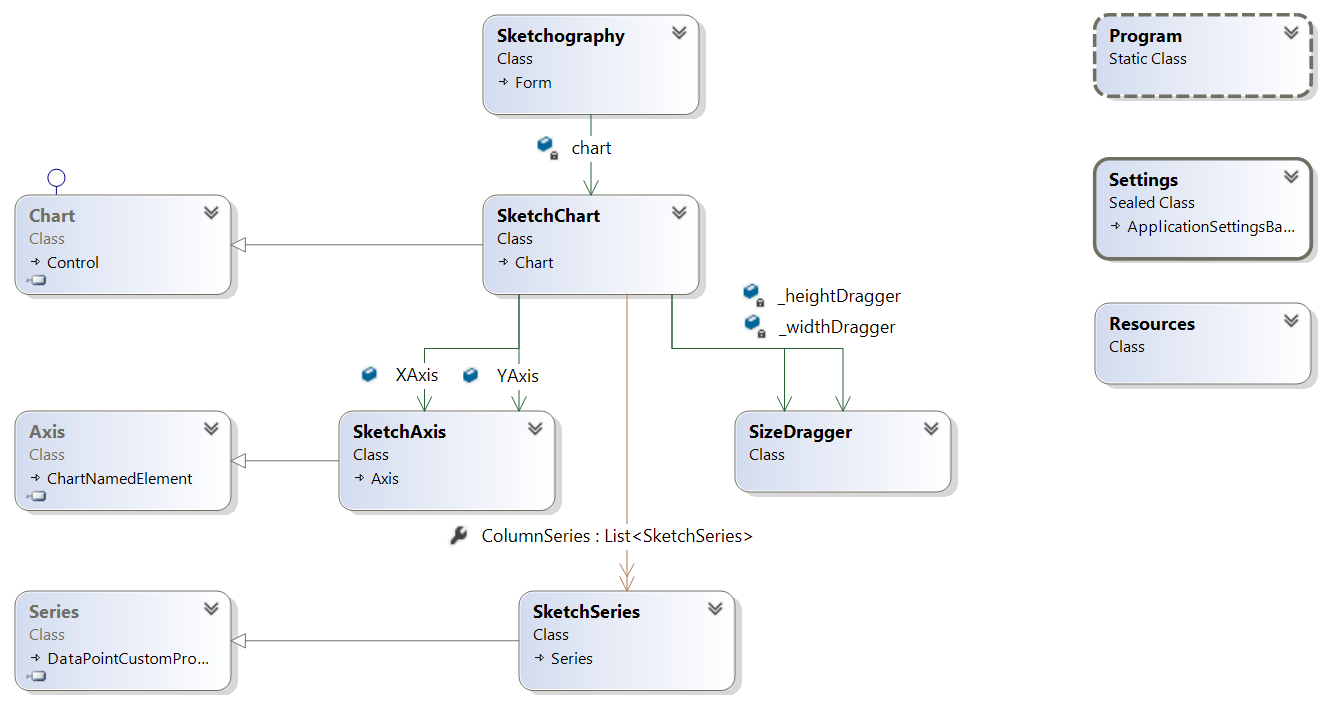
\includegraphics[width=1\linewidth]{ClassDiagram}
		\caption{Interactions between classes}
	\end{figure}		
	
	As seen above, the Sketchography form is the main application run when Program starts. Sketchography contains a SketchChart component, which contains the canvas for users to sketch on, as well as the formal chart generated. SketchChart in turn uses SketchAxis and SketchSeries objects. SketchChart, SketchAxis and SketchSeries inherit from their non-sketch counterparts Chart, Axis and Series (from System.Windows.Forms.DataVisualization.Charting, which is part of the .NET framework), in order to reuse the built-in functionality and members, and complement them with functions and members specific to sketching. SketchChart also references two instances of SizeDragger, which is a custom UI widget to support dragging ends of columns in a column chart to scale them. Settings and Resources are two additional classes used to store properties of the project.
	
	
	%TODO Should I include that the core of the project is around 620 lines of code? This doesn't include the classifier or the interface code
	No class is more than 400 lines of code, indicating that functionality has been split up at a reasonably fine grain to not concentrate too much responsibility in any one class. Visual Studio's calculated code metrics show that the project has a maintainability index of 74/100, which gets the highest rating - 'good' maintainability. Should I include the data in this paragraph?
	
	At a high level, the functionality of the program can be divided into 3 responsibilities - data handling, sketch processing and charting (in increasing order of complexity). It is written in an Object Oriented fashion, with separation between the views (Windows Forms) and controllers (C\# classes), to allow for easy testing.
	
	
	\subsection{Data import and management}
		Since the application is targeted at the average user, their data is most likely to be stored in spreadsheet format. Thus, it is important to allow them to import data from .xlsx and .csv files. 
		For the sake of simplicity, the code assumes that the data is well-formed. Specifically, it works on the following assumptions:
		\begin{enumerate}
		\item The data is arranged as records in the rows of the spreadsheet.
		\item The first row contains the names of the various fields.
		\item No data is missing (if there are $m$ columns and $n$ rows, there are $m \cdot n$ data values.
		\end{enumerate}
		
		Under these assumptions, importing tabular data is a common use case, so I studied a number of existing libraries and methods to do this in C\#. At first the LinqToExcel package from the NuGet package manager was used to easily import data from the file. However, this package had limited documentation, making it hard to achieve more complex tasks. Additionally, it added an external dependency, and carried a license that allow free reuse of the software as long as the original copyright message was included. The package was helpful for rapid prototyping at first, but after the code was more mature, we removed this dependency and implemented the file import ourselves using the OLE DB provider.
	
	%TODO Try to lay these screenshots out better, and decide whether first 2 are needed at all.
	\begin{figure}[h]
		\centering
		\begin{subfigure}[b]{0.3\textwidth}
			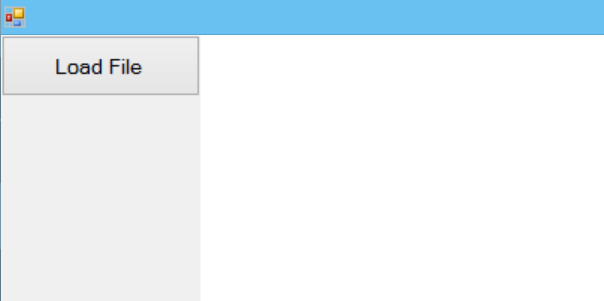
\includegraphics[width=\textwidth]{data1}
			\caption{Initial state}
			\label{fig:data1}
		\end{subfigure}
		\begin{subfigure}[b]{0.6\textwidth}
			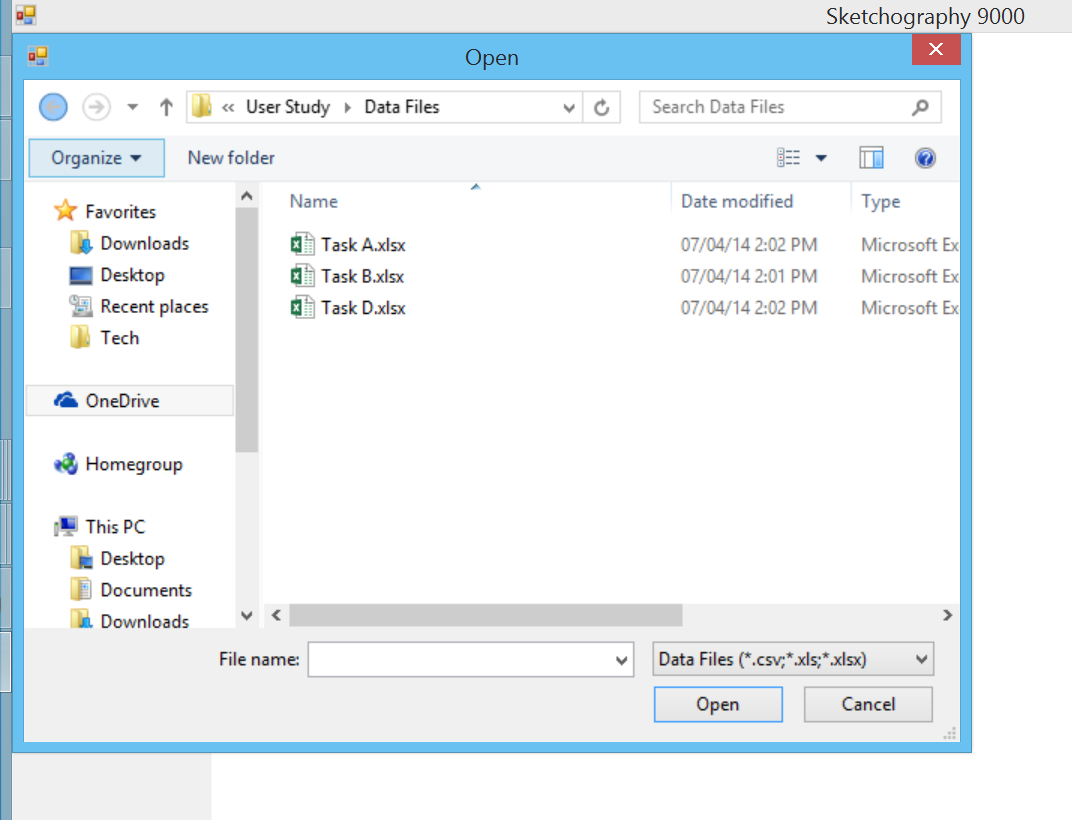
\includegraphics[width=\textwidth]{data2}
			\caption{When "Load File" is clicked}
			\label{fig:data2}
		\end{subfigure}
		\begin{subfigure}[b]{0.5\textwidth}
			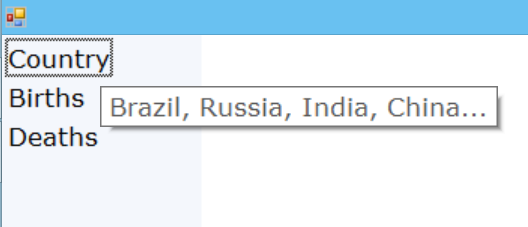
\includegraphics[width=\textwidth]{data3}
			\caption{Column headers are shown with data previews in tooltips}
			\label{fig:data3}
		\end{subfigure}
	\end{figure}		
		
		
	The interface shows a "Load File" button, which when clicked reveals a standard system filepicker dialog with a filter to show *.csv, *.xls and *.xlsx files.	Selecting a file causes the "Load File" button to disappear and be replaced by a list of column headers (the names of the various fields). This helps minimise interface clutter and only expose the most relevant information at all times. However, it comes at the cost of the user needing to hit 'Reset' if they choose the wrong file by mistake. To reassure the user that data has been imported correctly, and for them to check which column header corresponds to which data, hovering over any header reveals the first few entries for that field as a sample.
	
	
	\subsection{Sketch Processing Workflow}
	RATA.SSR provides a sample that calls the classifier API. For this project, that reference was followed, with a lot of extraneous code and unnecessary branches removed, until a basic prototype existed consisting of nothing but a blank canvas which receives user ink, passes it off to a classifier, and outputs the recognition result in a log-like text box. This was then integrated into the application described above, with its data import facility. 
	
	When the user draws a stroke on the SketchChart element within the Sketchography window, a number of steps occur:
	\begin{enumerate}
	\item The \texttt{SketchChart} is covered by an \texttt{InkOverlay} object, which receives the stroke. An \texttt{inkOverlay.Stroke} event is fired, which allows our event handler to run custom code.
	\item The \texttt{InkOverlay.Stroke} event handler calculates additional features of the stroke that are not included in the stroke's properties by default, and stores them in its extended properties.
	\item The stroke is then sent to the classifier, which is loaded from a file on program initialization.
	\item The \texttt{classifierClassify} function returns a string from a set of previously defined strings representing the various recognition results. This string is passed off to the \texttt{ConvertToFormal} method, which, as the name suggests, creates the corresponding formal chart elements. The \texttt{ConvertToFormal} method is also sent the stroke object itself, so that it can use its properties such as the location to place the formal object accordingly.
	 
	\end{enumerate}

	After the core of the project was finished, an extension was implemented that allows erasing of strokes. The stylus available has a button simulating an eraser at the back. When this eraser comes into range, a \texttt{CursorInRange} event is thrown, wherein we can check whether the stylus is inverted or not.
	
	\begin{lstlisting}[frame=single]
_inkOverlay.EditingMode = e.Cursor.Inverted ? 
		InkOverlayEditingMode.Delete : 
		InkOverlayEditingMode.Ink;
	\end{lstlisting}
	
	Then, when a stroke is received (the same event is thrown whether the stroke is ink or the eraser), if the editing mode is Ink, the steps above are run. If it is Delete, the corresponding chart element is detected and reset. On the next re-paint of the interface, this element will be removed from the canvas. To minimize lag between the action and the feedback, this repainting is forced immediately with an \texttt{Invalidate()} call.
	
	 Below is a description of how \texttt{ConvertToFormal} responds to user actions it receives, via the stroke classifier. 
	
	\begin{tabular}{p{0.2 \linewidth} p{0.8 \linewidth}}
	\bfseries User Action	& \bfseries Application Response \\
	Load File &
	Bind chart's data source to the in-memory data table created from the imported file. 
	\\
	
	\vspace*{10\lineskip}
	Draw an axis &
	\begin{enumerate}
	\item Calculate the bounding box (the smallest rectangle that entirely encloses the stroke) of the sketched axis, and use a heuristic comparing the height to the width to determine whether it is a vertical or horizontal axis. 
	\item The line running through the center of the bounding box is taken as the intended coordinates of the formal axis. This must be done since sketched axes are rarely perfectly straight lines, so using the actual endpoints of the line might result in a non-aligned axis. 
	\item The endpoint coordinates of the straightened line are used to set the vertical or horizontal position and size of the formal chart. They are also saved in an Axis object, which can then be drawn onto the formal chart.
	\item If it a horizontal axis, a drop target is below the axis. This is a rectangle of the same length as the axis, and a preconfigured height deemed big enough to make it hard for the user to miss, while minimising the screen space used up.
\end{enumerate}		
	\\
	
	\vspace*{10\lineskip}
	Draw a bar &
	\begin{enumerate}
	\item A bar is the indicator that the user wants a new data series added on a bar/column chart. Thus, a new data series is added to the chart's SeriesCollection in the form of a Series object. The name of this series is set as ``SeriesX'', where X is incremented for each new series. This will be useful for the drop target system described later.
	\item When the new series is added, the Chart object automatically assigns it a new series colour from the colour palette. The application changes the colour of the stroke the user drew to this series colour, to give feedback that it has been recognised as a series. 
	\item A drop target the same size and position as the bounding box of the bar is created, corresponding to that series.
	\end{enumerate}
	\\
	\end{tabular}

	\begin{figure}[h]
		\centering
		\begin{subfigure}[b]{0.4\textwidth}
			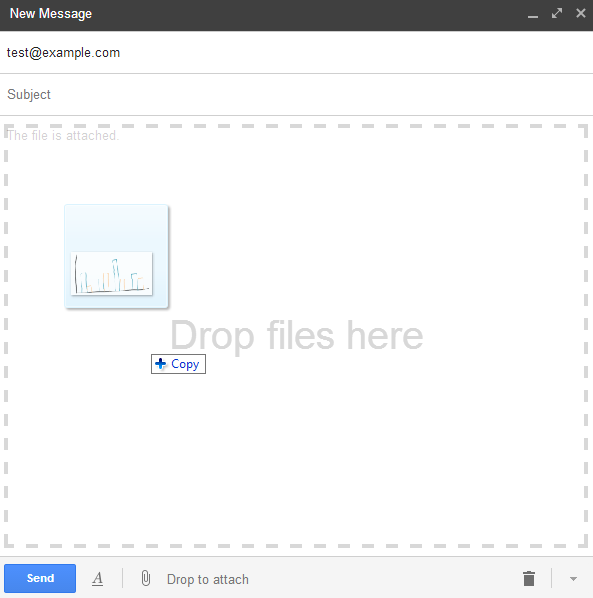
\includegraphics[width=\textwidth]{dropexample1}
			\caption{Gmail.com compose window, taken in May, 2014}
			\label{fig:dropexample1}
		\end{subfigure}
		\begin{subfigure}[b]{0.4\textwidth}
			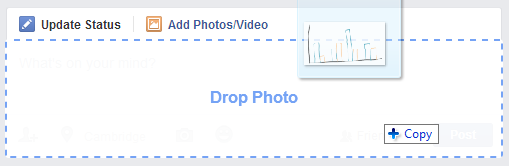
\includegraphics[width=\textwidth]{dropexample2}
			\caption{Facebook.com status update widget, taken in May, 2014}
			\label{fig:dropexample2}
		\end{subfigure}

	\end{figure}
	
	In response to strokes that create chart elements, drop targets are generated so that the user may then drag and drop data directly onto the chart element to bind it. This provides direct manipulation, since it doesn't force the user through a menu and dialogue system to configure which data corresponds to which axis. In order to do this, a dictionary is maintained in SketchChart, storing the mapping between Rectangles encoding the location of a drop target, and the string representing the chart element it corresponds to. For the x axis, this would be ``X Axis"; for the data series it would be the name of the series. 
	
	\begin{figure}[h]
	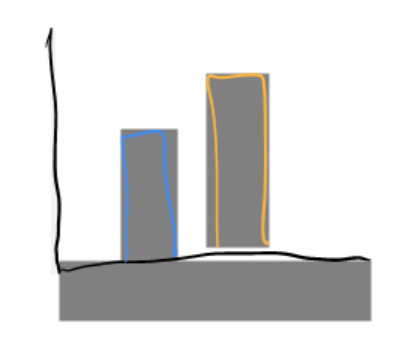
\includegraphics[scale=1]{droptargets}
	\caption{Drop Targets for 2 data series and the X axis, revealed when data is being dropped onto the chart}
	\end{figure}
	
	When the user begins dragging a column header from the list on the left, this calls a number of event handlers in Sketchography. These configure the drag and drop action so that the column name saved within the list item is the data sent to the drop location. They also flip a \texttt{ShowDropTargets} flag, so that the chart rendering system draws grey rectangles indicating where the drop areas lie. This UI pattern is based on one users may be familiar from a number of drag and drop interfaces they may have previously interacted with, thus making it easier for them to understand what's happening. We also tried adding `Drop here' text in the targets like in the examples below, but this proved to cluttered in the small drop targets being used. Additionally, hallway testing revealed that once users began dropping, they were already aware that they must drop it in targets, and the change in colour was conspicuous enough to draw their attention to them.
	
	When the data is dropped, this calls another event handler. In Sketchography, the event handler simply verifies that its a valid drag and drop, and then passes on the data to the \texttt{DropData} function on the SketchChart. For every rectangle in the dictionary of drop targets, \texttt{DropData} checks if the drop event occured within it. When it finds the drop target the user picked, it looks up the corresponding string, and calls \texttt{BindDataSeries} on it. \texttt{BindDataSeries} adds the binding appropriately. If the data was dropped on a data series rather than the X axis, it also renames that series and the corresponding drop target, so that the user can reassign that bar to some other data if they change their mind. From this point, the charting functionality takes over.
	
	
	
	
	

	
	\subsection{Charting}
	This part of the functionality, unexpectedly, proved the most challenging and time-consuming. In the first few iterations, a built-in .NET chart component was used, which allowed rapid prototyping. However, converting from the coordinate system used within the charting component to that used in the rest of the window was proving non-trivial and inaccurate. In addition, the component didn't allow very fine-grained positioning of its various elements, or much control over their sizing and other attributes. Hence, we had to implement our own chart control. To make the most of the functionality already implemented in the built-in control, we inherited from it. This also meant our custom control could easily replace the built-in one since it implemented the same interface but with a few extra features.
	
	The painting of the chart graphics is done in a largely procedural fashion unfortunately, as this is how it is done for Windows Forms controls. Most of the work is done in the \texttt{PostPaint} event handler, which is called after the built-in chart is done painting (even though the built-in chart control is not shown to the user at all, it still needs to be painted in a hidden background for some of its functionality to work correctly). This painting occurs whenever changes are made that might affect its output. Within the event handler, there are distinct sections that:
	\begin{itemize}
	\item Draw a background to cover up the built-in chart.
	\item Draw the formal axes and bars.
	\item Draw a height drag handle if needed.
	\item Draw a width drag handle if needed.
	\item Move the user's strokes to fit the bars.
	\item Draw the drop targets if needed.
	\item Change the colour of ink strokes to match their series colour if needed. 
	\item Update the legend.
	\end{itemize}
	
	Each of these steps involves a lot of complicated computation, maintaining of state, and conversion between coordinate systems. The particularly interesting parts are described below.
	
	\subsubsection{Positioning and scaling bars}
	To allow maximum flexibility, constants are introduced that control various parameters of the appearance of the bars, such as the ratio of the gap between them, and the fraction of the height of the chart they should cover by default. Then, formulae are used to account for the number of data series, the relative width scale of each series, the relative scale of the gap between data points, and the length of the X axis, to calculate the position each bar should be drawn at.
	
	The application also has to calculate the values to show for labels on the Y axis. This is something that the custom charting control doesn't handle as elegantly as the built-in control, since the values are not usually rounded, whole numbers. This is because the range of values in the data series is simply spread across a set number of labels to determine the individual label values.
	\subsubsection{Transforming strokes to match formal bars}
	\begin{figure}[h]
		\centering
		\begin{subfigure}[b]{0.35\textwidth}
			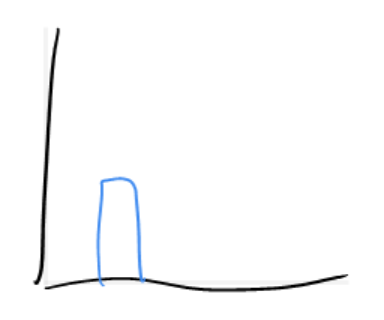
\includegraphics[width=\textwidth]{sketchtransform1}
		\end{subfigure}
		\begin{subfigure}[b]{0.4\textwidth}
			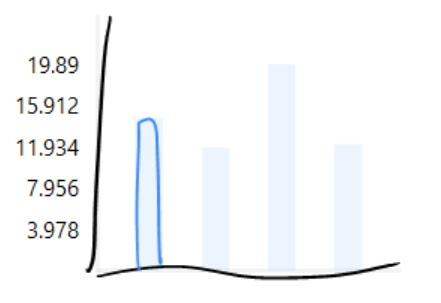
\includegraphics[width=\textwidth]{sketchtransform2}
		\end{subfigure}
		\caption{Before and after the transform}
	\end{figure}		
	
	This was implemented as an extension, to better express the connection between the sketches and the formal bars to the user. It is done by maintaining a mapping between the sketch and the first bar of the series. When the bar is drawn, its coordinates and dimensions are saved. These are then applied as a scale and translation transform to the associated sketch.
	
	
	\subsubsection{Height and width dragging}
	Another extension was to allow users to make changes to the formal chart, and have those changes feed back to the sketches. We decided to offer the ability to change the width and height of the bars. When in the formal view, if users hover over the first bar in a series, they see a drag handle each for the height and width, in the form of a grey rectangle. We decided on the size of these handles by experimenting with various sizes to see which one formed a target big enough to grasp with a stylus. Since these rectangles are simply graphics drawn onto a picture box rather than explicit controls, they do not offer native drag functionality. Instead, this has to be approximated by toggling a flag when mouse/stylus is down within the rectangle of the drag handle indicating that a drag has started. When the mouse/stylus is lifted, if the flag was on and the cursor position has changed, this is viewed as a drag, and the change in position is taken to be the size change desired. This scaling is then applied to the variables previously introduced for positioning and scaling bars, so the changes take effect in the next paint cycle, which seems fairly instantaneous to users, if not perfectly so.
	
	\begin{figure}
	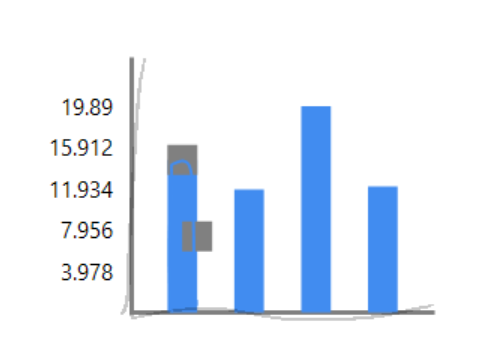
\includegraphics[scale=1]{draghandles}
	\caption{Drag handles}
	\end{figure}		
	
	To help users discover what these drag handles do, the cursor changes to a sideways drag cursor in the direction corresponding to whether it is a height or width handle, when it hovers over these handles.	
	
	At first, the naive implementation of the scaling broke when users tried particularly extreme drags, which they tended to play with even if it wasn't the scale they finally intended to use. The calculations had to be refined over time.
	
	\subsubsection{Maintaining the legend}
	To keep the user aware of the state of the system at all times, it is important to have a legend showing which data is connected to which element of the visualisation. While most charting tools have a separate legend, we decided, in the theme of direct manipulation, that the colour key should be right where the data is - in the list of column headers. 
	
	However, the list of column headers is in the Sketchography form, whereas the colours are stored within the SketchChart, which is referenced in the form. We followed a subscriber pattern here, by creating an event in SketchChart that notifies about changes to the legend. SketchChart also exposes a public Legend dictionary, mapping colours to headers. Sketchography subscribes to those notifications, and its event handler regenerates the legend by checking the list in SketchChart.	
	
	\begin{figure}
	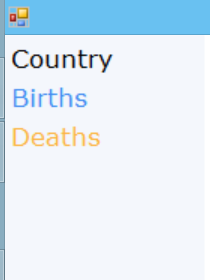
\includegraphics[scale=1]{legend}
	\caption{Legend}
	\end{figure}
	
	
	\subsubsection{Switching between the formal and informal views}
	We initially did this by offering a simple toggle button that read `Toggle View', and a text box that showed the current view the user was in `Sketch View' or `Chart View'. However, during hallway testing, users repeatedly clicked on the text box, or were just generally confused about which view they were in. This confirmed a previous worry that the disconnect between the action trigger and the reflection of its actions would be confusing, so we implemented radio buttons as shown below. These contain pictures of the two views, so users can spot the difference visually without needing to internalise what the two phrases represent. Another concept of showing visual layers with live previews was not tested because of time and technical constraints.
	
	%TODO Get screenshot of earlier iteration
	
	\begin{figure}[h]
	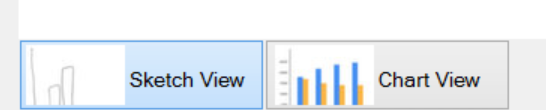
\includegraphics[scale=1]{toggle}
	\caption{Switching between formal and informal views}
	\end{figure}
	
	Behind the scenes, all the chart elements are drawn in both views, with the unselected view dimmed or ghosted out. Hence, when users are sketching, they can see faint feedback of the recognition in the background and thus notice early if there has been a misclassification. This is done by setting two alpha or transparency values - one which is high when the formal view is selected, and one which is high when the in informal mode. Each of the elements then uses one of these alpha values to draw themselves according to which mode they should be prominent in.
\chapter{Evaluation}
Given that design usability was the salient point of this project, a user study was a good way to assess its performance. After gaining approval from the Ethics board, a pilot study was run, followed by the actual user study. The results confirm the hypotheses - users learnt how to use the system after one use, and they were able to modify their chart faster in Sketchography compared to Excel. A description of the study and a summary of the results follows; for the entire questionnaire and full data analysis, see \autoref{cha:questionnaire} and \autoref{cha:analysis}.
%TODO Add reference to appendix ^
%TODO Maybe add a qualitative example here of horribly drawn charts being correctly identified. Or atleast mention that the recognition works remarkably well.

\section{Study Goals}
In the Introduction (\autoref{cha:introduction}), I hypothesized that the direct manipulation and liveness of this system would offer two advantages:

\begin{enumerate}
\item[H1] This interface is more `learnable' over time
\item[H2] It encourages exploratory data visualisation creation by making modification easier
\item[H3] Its advantages hold independent of how fluent the user is in English.
\end{enumerate}

The study was designed to evaluate whether these three properties were achieved. 

\subsection*{Learnability}
To investigate whether the interface is learnable over time, users were asked to carry out a very similar task twice, and their times across tasks were compared. If the user shows a statistically significant improvement in the time taken to carry out the task, then they are learning how to use the interface, and becoming adept at using it. The chosen task is to import (mock) data and create a bar chart.

To make this experiment fair, the tasks had to be phrased very carefully. The tasks had to be very similar, to make sure one was not systematically harder or easier, but not so similar that users could mechanically follow the same steps without even understanding the problem.

In addition, the tasks had to tell the user what output is expected, without explicitly listing every single step required to get there. This did not hold true for the version of the task descriptions used in the pilot, an example of which is below.

\begin{quotation}
Task A:
\begin{enumerate}
\item Load the `Task A.xlsx' file.
\item Create a bar chart of `Births' and `Deaths', with `Year' on the X Axis.
\end{enumerate}
\end{quotation}

Clearly, this would leave little room for users to demonstrate that they have learnt how to use the application, since the task guides them through exactly what they need to do. Thus, the task was rephrased to focus on the problem (note, the data schema of the file was also changed to focus on differences between countries rather than years).

\begin{quotation}
Task A:

You work in a government agency and are trying to see how population is growing in 4 different countries. The ‘Task A’ file contains information regarding how many births and deaths occurred in 1 year in each country (the numbers are scaled to account for population). 

Use the Sketchography app to create a column bar chart that will allow someone to compare birth and death rates across the countries.

Speak out aloud the name of the country where the population is declining (where the death rate is larger than the birth rate).

\end{quotation}

This is better, since the user now needs to understand the context of the problem, grasp which data is relevant and which fields need to go on each axis for them to notice the trend required.

\subsection*{Modification}
To see whether the interface enables quick exploration, the time required to make a specific modification in Sketchography needed to be compared to the time required for the same modification in users' usual chart editor. The only other chart editor we compared was Microsoft Excel, which proved a sensible decision since all the final study participants indicated that Excel was their tool of choice for making charts, and only 2 out of 10 had actually used anything else to create a chart.

To make the comparison fair, we needed a modification that was a reasonable change to make quickly, and was supported by both editors. Two such changes are to change the width of the bars, and to change the height of the bars, without changing the dimensions of the chart itself. In the pilot study, some participants were asked to change the height, while others were asked to change the width. However, in Excel, the user has no direct control over the width of the bars. Instead, they have to do this indirectly by changing a 'Gap Width' setting, which controls the space between the bars. This indirection was not a perfect analogue to the method to change the bar width in Sketchography, so some users never identified how to make this change. Thus, in the final user study, we focused instead on changing just the height of the bar, which could be done via similar settings in both applications.

The users weren't shown how to make this change, or that the option was only available in the formal view (since stylus interaction with the chart in sketch view would be interpreted as ink). They had to explore the User Interface and discover the way to do this themselves. The method involved hovering over a bar in the data series, which exposes a drag handle on the top and the right of the bar. The top one can be dragged to manipulate the height (more specifically, the Y axis scale). In Excel, it involved opening an `Action Pane' by double clicking on a bar, or right clicking on it and then selecting the right option, or via a button in the ribbon interface on the top of the screen. In this `Action Pane', there was a setting to change the Y axis scale.

\subsection*{Language Independence}
A secondary benefit of the direct manipulation and visual metaphors is that Sketchography isn't as language dependent as a system with configuration dialogues in English. Users should be able to learn Sketchography just as quickly whether they speak English as their primary language or not. 

India is a nation of multiple languages, but a lot of businesses conduct their activities in English. By carrying out the study there, participants with varied levels of fluency in English can be recruited.

To study the effect of language on the two measures above, users were asked what their primary language was, on their questionnaire. This was then divided into a binary classification: English or Non-English.

\subsection*{Other factors}
A number of factors could affect people's performance on these tasks. For example, users who regularly create charts in Excel might be able to do so faster. To investigate how these factors affect the measures above, a questionnaire was given to users following their completion of the tasks, asking:

\begin{enumerate}
\item How often do you make charts for work or studies?
\item What tool do use for making these charts?
\item How many years have you been using that tool for?
\item Have you used Microsoft Excel to make charts?
\end{enumerate}

Additionally, participants were asked three open-ended questions to gain qualitative observations on their thoughts on Excel and Sketchography.

The exact phrasing of the task descriptions and the questionnaire is in \autoref{cha:tasks} and \autoref{cha:questionnaire} respectively.


\section{Pilot Study}
The pilot study was conducted with 3 participants, all graduate students (aged between 20 and 30) at the University of Cambridge Computer Lab, who were not paid for their time. They were members of the Graphics and Interaction group, and had carried out user studies of their own in the past. Besides directly contributing as participants in the study, they could also help me identify any flaws in the study setup. The study was carried out in a controlled lab environment, with equipment that recorded video of participants' interactions with the application, and audio of what they were saying as they interacted with it.

The study proceeded as follows:
\begin{enumerate}
\item The participant signs a form indicating his consent to participating, and being recorded for the purposes of the study. They are also informed that they are being timed not to assess their own performance, but that of the system, in order to put them at rest.
\item I demonstrate the system to them by importing a data file, creating a bar chart, switching between formal and informal views and resetting the application to its initial state.
\item I explain that they will be given a task description on a slip of paper, and can take as long as they like to read it. When they are ready, I will start timing. While they are carrying out the task, I will provide no assistance, in order to maintain uniformity.
\item The Surface tablet is presented to them, with the application open in its initial state. The default folder when the `Open File' dialogue is opened contains only the three Excel files they need for their tasks, and are named `Task A.xlsx' and so on.
\item They are given the 2 creation tasks, followed by the two modification tasks. Comments they make out loud during this time are noted down. 
\item After they finish all 4 tasks, they are given the questionnaire.
\item After they finish the questionnaire, they are free to leave. Most stay to make comments about the software, which are also noted down.
\end{enumerate}

The key things learnt were:
\begin{enumerate}
\item The task descriptions gave the steps in too much detail, as described above.
\item The width modification task was not appropriate, as described above.
\item Despite it being subtly mentioned that each chart element must be drawn with an individual stroke, some users draw both the X and Y axis in one stroke as an `L' shape. The program is modified before the final study to recognise these axes correctly and instantiate the two Axis objects accordingly. 
\end{enumerate}

There were no structural issues with the way the study itself was carried out, but the timing techniques and the script used during the demonstration did get refined with practice, making for a more valid final user study.

\section{User Study}
The final user study was conducted with the same structure as the pilot study since no issues were faced. To get a fair mix of native and non-native English speakers, it was carried out in Mumbai, India. 10 participants with various levels of experience with Excel, and aged between 20 and 60 years old, volunteered. They were all white collar workers in various industries, some of whom used computers on a daily basis.

\begin{table}
\begin{center}
\begin{tabular}{c c}
Age group & Number of participants \\
20-30 & 4 \\
30-40 & 1 \\
40-50 & 4 \\
50-60 & 1 \\

\end{tabular}
\end{center}
\caption{Distribution of participant ages}
\end{table}

One issue that the pilot study did not identify but was highlighted in the user study was the different ways people draw bars. Some of the Indian participants drew bars as two strokes, which none of the English participants had done. Thus, one of the strokes making up the bar would get recognised as an axis rather than a bar. This led to some interesting observations. The program has the ability to erase and redraw strokes that have been misclassified. However, for the purposes of the study, this feature was not demonstrated to users for 2 reasons:
\begin{enumerate}
\item The eraser is one of the less discoverable aspects of the application. Any of the participants could have noticed the eraser like shape at the end of the stylus and tried pressing it. I wanted to see if any users would discover this on their own, without being shown. None of the 10 did so, presumably because users have previously been familiar only with capacitative styluses that don't have such a feature. 
\item No matter how robust the stroke recogniser is made, there will be classification errors during usage. It was important to note how users react to this, understand what has happened, and correct the problem.
\end{enumerate} 

In practice, each of the users who made these split bars found a way around this. One took the less desirable option of hitting `Reset' and starting over, but the majority just drew over their previous sketches. When a new axis was drawn, the old, misinterpreted one was forgotten, and the chart got corrected. Then, the user would draw the bar with one stroke as required.

\subsection{Learnability}
Our hypothesis was that the time taken for the creation task the second time around would be lower, and this was confirmed by a Paired T Test as shown below.

%TODO Either change all commands to colour or change this back to black.
\begin{alltt}
> \hlkwd{t.test}\hlstd{(Task1, Task2,} \hlkwc{paired} \hlstd{=} \hlnum{TRUE}\hlstd{)}
\end{alltt}
\begin{verbatim} 
	Paired t-test

data:  Task1 and Task2
t = 5.2186, df = 9, p-value = 0.0005502
alternative hypothesis: true difference in means 
is not equal to 0
95 percent confidence interval:
 23.34058 59.05942
sample estimates:
mean of the differences 
                   41.2 
\end{verbatim}

%TODO Add boxplot and/or table showing mean/median differences.

The null hypothesis in the Paired T Test is that there is no difference in the Task 1 and Task 2 times for each participant. A $p-value < 0.05$ is considered to show that the two distributions are significantly different, and therefore the null hypothesis can be rejected. For every participant, there is a statistically significant difference in times between Task 1 and Task 2 - they were on average 41 seconds faster on their second try. The test is valid if the data follows a normal distribution, which a Q-Q plot and Shapiro-Wilk test suggested holds for this data.

\begin{table}[H]
\begin{center}
\setlength{\tabcolsep}{8pt} 
\renewcommand{\arraystretch}{1.5}


\begin{tabular}{l | l l}
Dataset & W & p-value \\ \hline
Task 1 & 0.8435 & 0.04854 \\
Task 2 & 0.8317 & 0.03511 \\
\end{tabular}
\end{center}
\caption{Creation task data was normally distributed}
\end{table}


\subsection{Modification}
The hypothesis was confirmed that people took significantly less time to modify the chart in Sketchography than they did in Excel.

A Paired T Test show this to be true ($p-value = 0.001389$), but was inconclusive since the data was not normal in this case ($p-value = 0.3966$ for Sketch and $0.1896$ for Excel). 

\begin{figure}[H]
		\centering
		\begin{subfigure}[b]{0.4\textwidth}
			\includegraphics[width=\textwidth]{figure/sketchqq.png}
		\end{subfigure}
		\begin{subfigure}[b]{0.4\textwidth}
			\includegraphics[width=\textwidth]{figure/excelqq.png}
		\end{subfigure}
		\caption{Modification task data wasn't normally distributed}
	\end{figure}

A Wilcox test, which doesn't rely on the same assumptions of normality, confirmed the hypothesis true. On average, each participant took 56 seconds fewer in Sketchography than in Excel.

\begin{verbatim}
	Wilcoxon rank sum test with continuity correction

data:  Sketch and Excel
W = 15.5, p-value = 0.01014
alternative hypothesis: true location shift is not equal to 0
\end{verbatim}

Qualitatively, a lot of participants were observed trying to drag the bounding box handles that appear when you select a bar in the Excel chart. They were frustrated when they realised that these handles can't actually be manipulated. One participant seemed to have prior experience with this - on reading the task, they said out loud, ``Oh yeah this is a pain, I know this is a pain".

Even when users did find relevant options in the Excel configuration panels, three of them hovered over the button, hesitated, and then tried something else instead. One actually said ``But this is different, no?", before abandoning it. They weren't able to instantly preview what result they would get if they picked the button, so they avoided exploring that possibility. 

On the other hand, they felt comfortable dragging the height handle in Sketchography despite it not having a label confirming its purpose.

One user even tried using the interface with a mouse, and by pinching her fingers apart on screen in a `zoom in' gesture. This suggests a willingness to experiment. It also suggested some future work for this project, to integrate finger gestures to manipulate the chart while using the pen purely for inking.

\subsection{Language Independence}
Half the participants spoke English as their primary language with native fluency, while the other half used it during their job but not as a primary language. Tests to show that the learnability for English speakers was more than that for non-English speakers failed. While not statistically conclusive, this suggests that there wasn't a significant difference in learnability depending on language, which supports the hypothesis.

\subsection{Other observations}
Given that some participants might have a lot of experience with Excel and none with Sketchography, making it an uneven playing field, data was collected about how frequently they use Excel. As might be expected, the less frequently the participant used Excel, in general, the bigger the gain in speed they got from using Sketchography for the Modification task. There aren't enough samples per frequency category (Daily, Weekly, \ldots) to run a conclusive statistical analysis, but the trend is visible in \autoref{fig:frequencybox}.

\begin{figure}[H]
\begin{center}
\includegraphics[width=0.8\linewidth]{figure/frequencybox.png}
\end{center}
\caption{Less frequent users of Excel gain a bigger speedup from using Sketchography}
\label{fig:frequencybox}
\end{figure}


No correlation was observed between the creation time task difference and the number of years the participant had used computers (Pearson's product-moment correlation $p-value = 0.1978$). Similarly, there was no correlation between creation time difference and the years of Excel use($p-value = 0.1386$).  

Interestingly, there is no correlation between the modification tasks time difference and whether the participant has used Excel for charting ($p-value = 0.5753$). This suggest that users might still not have learnt how to use Excel after having used it before, unlike Sketchography where they showed a measurable speedup after having used it once.

\subsection{Participant comments}
Some of the interesting responses to the open-ended questions are included below.

\textbf{Question: How do you think the software works?}

(Note: This question intended to elicit whether the participants had formed a correct mental model of how the software functions, but some of the participants less averse with English misinterpreted it as soliciting feedback, which led to even more interesting answers)

``Easy and real fast."

``Works pretty well. It is much easier to understand this software as compared to Excel."



\textbf{Question: What is the best thing about Excel?}

``Can easily plot the data and could be understood easily."

``All pervading."

\textbf{Question: What is the worst thing about Excel?}

``Certain times it is time consuming."

``Too vast to remember everything."

``Flexibility in charts is fairly low - it's templatized for the most part and not customize-able."

``Cumbersome."


\textbf{Question: What is the best thing about Sketchography?}

``Very efficient software. Easy to understand. Charts can be prepared in a matter of seconds."

``Intuitive."

\textbf{Question: What is the worst thing about Sketchography?}

``While making bars, not everybody will have the same style, so the Y Axis can get misjudged. Rest was easy and fun. Less time consuming. User friendly. Mistakes should get highlighted."

``The image recognition could be better. Apart from that, the software is easy to use, extremely intuitive, versatile and has great potential."

``A few kinks to work out, but on the right track."

\section{Summary}
In the introduction, this project outlined some hypotheses that it believed would be supported by the merits of the application. This chapter details a user study carried out on 10 participants that confirmed the two primary hypotheses with statistically significant results, and suggested that the third is supported too. Namely, users learn how to use the software on their first try and are already becoming skilled, and thus faster on their second try. They are also able to determine how to make a specific change quicker in Sketchography than they are in Microsoft Excel. It is likely that they have been able to learn how to use the application and make the modification regardless of how conversant they are in English.
\chapter{Conclusion}
Overall, this project went better than expected, resulting in three extensions being implemented. It was shown to be a statistically significant improvement over existing tools in terms of learning curve. This was the result of numerous design iterations, and a lot of code to develop the custom charting system that best matched the project needs.

\section{Comparison with Requirements}
The requirements (\autoref{sec:Requirements}) originally listed in the Preparation are restated below for verification that they were met and exceeded.

The system must allow the user to:
	\begin{enumerate}[label=\bfseries Core \arabic*]
		\item Visualise data they have stored in common file formats.
		\item Specify the type of chart they want by drawing a likeness of it on screen using a stylus.
		\item Bind the data to the chart using an interface that makes it clear how the data is being used to generate the graphics.
		\item Specify visual properties of the chart, such as size and position, through the sketches.
		\item Manipulate the visual appearance of the created chart.
	\end{enumerate}
	
	These core requirements were all met.
	In addition, time permitting, the system may:
	\begin{enumerate}[label=\bfseries Extension \arabic*]
		%TODO Make this first point clearer
		\item Transform user-drawn sketches to resemble and overlap the formal chart elements they generated, in order to show the link between the sketch and the formal elements visually.
		\item Mirror any manipulations applied to the formal layer back to the user drawn sketches, in order to keep the visuals of the formal and sketch layers in synchronisation.
		\item Allow users to undo actions by erasing sketches, and remove the corresponding formal elements without throwing errors.
		\item Allow users to manipulate any property of chart elements, not just one, so that the domain of visualisations they can create is infinite. For example, allow them to bind not just the height of bars in a bar chart to data, but also their width and colour. 
		\item Analyse the data and infer properties that may allow it to automatically suggest properties of the chart, such as which field belongs on which axis, or whether a data series should be log scale or linear scale.
		\item Support exporting the chart as a Microsoft Chart object that can be embedded as a dynamic object in Microsoft Office files, not just as a raster image.
	\end{enumerate}
	
	Extensions 1, 2 and 3 were implemented, resulting in an even better design. Extension 4 could have been built since most of the technical platform required already existed, but was decided against in order to keep the application simple for users to understand, and make it possible to make charts quickly.	
	
	Some usability goals were also specified:
	\begin{enumerate}[label=\bfseries Usability \arabic*]
		\item Users must be able to create charts at least as quickly as they can using current charting systems.
		\item Users must be able to build a mental model of the software's behaviour within 2 uses of it. They should thus be able to accurately predict the consequences of any action taken within the software.
		\item Changes to the visualisation must occur through directly manipulating the visual representation of the chart, rather than through disconnected User Interface widgets.
		\item The user must be able to easily try out changes to the visualisation, see what the resultant chart would look like, and undo them if needed.
	\end{enumerate}
	
	Anecdotally, users were able to create charts within minutes, and made comments about the perceived speed. The user study demonstrated that they had built up a mental model by correctly applying the understanding they had gained from one task, to perform a second, similar task quicker. All changes to the chart are made directly on the chart, there is minimal other UI. The second half of the user study demonstrated that the application could encourage exploration, since users made the same modification to their chart significantly faster in Sketchography than the leading charting tool, Microsoft Excel.
	
\section{Future Work}
While the goals of the project were met, the exploratory design phase as well as the user testing generated a lot of ideas that weren't feasible to implement within the time scale.

The primary improvement that would make this tool more practical would be to enable exporting the chart, as an image, or better yet, as a Microsoft Office Chart object that can be embedded as a vector object in office applications.

Additionally, the technical platform built could be extended to support many more types of charts. Given the small amount of data collected to train the classifier, adding recognition support for many more chart elements could have lowered accuracy, which would be detrimental to the usability. However, with more time, more data could be collected, for a variety of chart types.

The charting component could also be made a bit smarter, to apply heuristics such as shifting the axes slightly to make them align perfectly.

\addcontentsline{toc}{chapter}{Bibliography}
%\bibliography{refs}

\cleardoublepage

%TODO: Appendices go here
\chapter{Appendices}




Irrefutable evidence that users learnt how to use the software and got faster after one try.
%TODO Fix the width of this thing:
\begin{knitrout}
\definecolor{shadecolor}{rgb}{0.969, 0.969, 0.969}\color{fgcolor}\begin{kframe}
\begin{alltt}
\hlkwd{t.test}\hlstd{(Task1, Task2,} \hlkwc{paired} \hlstd{=} \hlnum{TRUE}\hlstd{)}
\end{alltt}
\begin{verbatim}
## 
## 	Paired t-test
## 
## data:  Task1 and Task2
## t = 5.219, df = 9, p-value = 0.0005502
## alternative hypothesis: true difference in means is not equal to 0
## 95 percent confidence interval:
##  23.34 59.06
## sample estimates:
## mean of the differences 
##                    41.2
\end{verbatim}
\end{kframe}
\end{knitrout}


The test is valid if the data follows a normal distribution. For each of the tasks, below is a Q-Q plot comparing the actual values (points) to the theoretical normal (line), and the results of the Shapiro Wilk test of normality.
	
\begin{knitrout}
\definecolor{shadecolor}{rgb}{0.969, 0.969, 0.969}\color{fgcolor}
\includegraphics[width=\maxwidth]{figure/unnamed-chunk-31} 
\begin{kframe}\begin{verbatim}
## 
## 	Shapiro-Wilk normality test
## 
## data:  Task1
## W = 0.8435, p-value = 0.04854
\end{verbatim}
\end{kframe}
\includegraphics[width=\maxwidth]{figure/unnamed-chunk-32} 
\begin{kframe}\begin{verbatim}
## 
## 	Shapiro-Wilk normality test
## 
## data:  Task2
## W = 0.8317, p-value = 0.03511
\end{verbatim}
\end{kframe}
\end{knitrout}



Similar evidence that people took longer to change the bar height in Excel than in Sketchography.

\begin{knitrout}
\definecolor{shadecolor}{rgb}{0.969, 0.969, 0.969}\color{fgcolor}\begin{kframe}
\begin{alltt}
\hlkwd{t.test}\hlstd{(Sketch, Excel,} \hlkwc{paired} \hlstd{=} \hlnum{TRUE}\hlstd{)}
\end{alltt}
\begin{verbatim}
## 
## 	Paired t-test
## 
## data:  Sketch and Excel
## t = -4.548, df = 9, p-value = 0.001389
## alternative hypothesis: true difference in means is not equal to 0
## 95 percent confidence interval:
##  -83.55 -28.05
## sample estimates:
## mean of the differences 
##                   -55.8
\end{verbatim}
\end{kframe}
\end{knitrout}



\begin{knitrout}
\definecolor{shadecolor}{rgb}{0.969, 0.969, 0.969}\color{fgcolor}
\includegraphics[width=\maxwidth]{figure/unnamed-chunk-51} 
\begin{kframe}\begin{verbatim}
## 
## 	Shapiro-Wilk normality test
## 
## data:  Sketch
## W = 0.9246, p-value = 0.3966
\end{verbatim}
\end{kframe}
\includegraphics[width=\maxwidth]{figure/unnamed-chunk-52} 
\begin{kframe}\begin{verbatim}
## 
## 	Shapiro-Wilk normality test
## 
## data:  Excel
## W = 0.8943, p-value = 0.1896
\end{verbatim}
\end{kframe}
\end{knitrout}


\bibliographystyle{apalike}
\bibliography{collection}
\end{document}
